\documentclass[10pt,conference]{IEEEtran}
\IEEEoverridecommandlockouts
\usepackage{cite}
\usepackage{amsmath,amssymb,amsfonts}
\usepackage{graphicx}
\usepackage{booktabs}
\usepackage{multirow}
\usepackage{xcolor}
\usepackage{tikz}
\usepackage{pgfplots}
\usepackage{pgfplotstable}
\pgfplotsset{compat=1.17}
\usepackage[hidelinks]{hyperref}

\def\BibTeX{{\rm B\kern-.05em{\sc i\kern-.025em b}\kern-.08em
    T\kern-.1667em\lower.7ex\hbox{E}\kern-.125emX}}

\begin{document}

\title{Routing Is Not Free: Latency and Cost of Query-Conditioned LLM Assignment}

\author{
\IEEEauthorblockN{Anonymous Author(s)}
\IEEEauthorblockA{Anonymous Institution}
}

\maketitle

\begin{abstract}
Query-conditioned routers are sold as a way to place each LLM request on the right cost--latency--accuracy point. We treat that claim as a performance-engineering hypothesis and evaluate it on a frozen 364-item panel with three backends (Qwen3.5-9B, gpt-oss-20b, gpt-4o) whose wall-clock HTTP round-trip times differ by more than an order of magnitude. Per-tier latency is heavy-tailed at the slow backend (T1 mean $42.47$\,s versus p50 $18.01$\,s, p90 $166.58$\,s; $n{=}364$ each). A deployed keyword router assigns $274/87/3$ queries to T1/T2/T3, so its \emph{policy} latency is a per-query mixture dominated by T1: mean $36.20$\,s, p50 $11.89$\,s, p90 $108.58$\,s. Always-T2 is simultaneously cheaper (\$0.0418 vs.\ \$0.2867), faster (mean $6.41$\,s, p90 $9.96$\,s), and more accurate ($92.3\%$ vs.\ $86.8\%$). That three-way domination holds in $99.99\%$ of $10{,}000$ item bootstraps, on every leave-one-benchmark subset, and in all $21$ mix-simplex cells. On the two-dimensional cost--latency hull of deployable policies, only Always-T2 and Always-T3 are undominated; the router is strictly interior. The result is a negative but actionable SLO lesson: a router that over-predicts ``hard'' (or, here, over-uses a verbose local model as the default tier) selects the \emph{slowest} backend, not the Pareto frontier. Static assignment to the empirically best backend is the baseline a router must beat. We report percentiles, not only means; latency is full HTTP RTT, not time-to-first-token.
\end{abstract}

\begin{IEEEkeywords}
LLM serving, query routing, latency tails, cost--latency Pareto, SLO, negative result
\end{IEEEkeywords}

\section{Introduction}

LLM serving is a performance problem before it is a modeling problem. Production stacks already differentiate prefill from decode~\cite{yu2022orca,zhong2024distserve,patel2024splitwise}, page KV cache~\cite{kwon2023vllm}, and schedule under SLO and goodput targets~\cite{agrawal2024sarathi,sun2024llumnix}. A second control loop has appeared at the \emph{model} layer: given a query, pick which backend to call. Cascades and learned routers~\cite{chen2023frugalgpt,ding2024hybridllm,ong2024routellm} are typically motivated as cost-saving devices. They are also scheduling policies. They change the mix of service-time distributions that the rest of the stack will see.

That mix is not a small perturbation. On the panel studied here, the three evaluation backends have mean HTTP round-trip times of $42.47$\,s, $6.41$\,s, and $1.14$\,s. The slowest backend's mean is more than twice its median; its p90 is $167$\,s. A router that sends three-quarters of traffic there does not add a lightweight decision hop---it \emph{selects a different service distribution}. Even if classifier time were zero (and on this panel it was not recorded), the assignment itself can dominate end-to-end latency.

This paper asks three performance questions. RQ1: are the three backends interchangeable SLO classes? RQ2: does the deployed assignment improve the cost--latency--accuracy Pareto set over static single-tier policies? RQ3: does that answer depend on the HumanEval/MMLU/GSM8K mix? We reconstruct the answers from a frozen three-tier Q\&A deployment (EcoLogic) with complete per-item, per-tier measurements ($n{=}364$: HumanEval, MMLU, GSM8K~\cite{chen2021humaneval,hendrycks2021mmlu,cobbe2021gsm8k}). We do not introduce a new scheduler. We measure whether an already-deployed keyword router beats the obvious static baselines on wall-clock latency and billed USD.

It does not. Always sending every query to the middle tier (gpt-oss-20b) Pareto-dominates the router on USD, mean and tail latency, \emph{and} accuracy. Always sending to gpt-4o is the low-latency, high-USD vertex. The router sits strictly inside that hull. We treat this as a useful negative result for LLMOps: the baseline a router must beat is static assignment to the empirically best backend, and ``best'' is a three-objective point, not a quality score.

\paragraph{Contributions.}
(1)~Per-tier latency distributions with p50/p90/p99, showing T1 is a tail-dominated outlier at similar seconds-per-output-token to T2.
(2)~Policy-level end-to-end latency reconstructed \emph{per query} from the selected backend's stored \texttt{latency\_s}, not from mix$\times$mean of tier averages.
(3)~A cost--latency scatter of deployable policies (marker size $\propto$ accuracy) whose two-dimensional hull is \{Always-T2, Always-T3\}.
(4)~An LLMOps implication: over-assignment to a verbose ``cheap'' model is an SLO anti-pattern, distinct from classifier overhead.
(5)~Tail-mass and labelled M/G/1 what-if numbers that convert a $5.6\times$ mean gap into a stability region: the deployed mix saturates below $100$\,q/h while Always-T2 remains stable past $200$\,q/h.

\section{Related Work}

\paragraph{LLM serving systems.}
Iteration-level scheduling in Orca~\cite{yu2022orca} and paged KV management in vLLM~\cite{kwon2023vllm} made high-throughput decode practical. DistServe and Splitwise disaggregate prefill and decode so the two phases do not share the same SLO envelope~\cite{zhong2024distserve,patel2024splitwise}. Sarathi-Serve chunked prefills to tame the throughput--latency trade-off~\cite{agrawal2023sarathichunk,agrawal2024sarathi}. FastServe, S-LoRA, Llumnix, and SGLang further specialize scheduling, adapter multiplexing, live migration, and structured decoding~\cite{wu2023fastserve,sheng2024slora,sun2024llumnix,zheng2024sglang}. Transformer serving at scale is also a batching and memory-bandwidth problem~\cite{pope2023efficiently}. None of these systems pick \emph{which model} to call; they assume the model is given.

\paragraph{Classical prediction serving.}
Clipper and Clockwork established that serving is an SLO and predictability problem, not only a throughput problem~\cite{crankshaw2017clipper,gujarati2020clockwork}. LLM routers inherit that framing once backends have unequal tails.

\paragraph{Tail latency and SLO serving.}
The tail at scale is a first-class performance object: a 99th-percentile delay that is rare on one call becomes typical in fan-out systems~\cite{dean2013tail}. Clockwork and Heracles treat p99 as the SLO to isolate, not a residual~\cite{gujarati2020clockwork,lo2015heracles}. Classical queueing design treats the service-time CV as a first-class input to waiting time~\cite{kleinrock1975queueing,harchol2013performance}. LLM routers inherit both problems once backends have unequal tails: a mix is a mixture of service-time distributions, the mixture's p90 is not the mix of p90s, and the mixture's CV---here $1.57$ for EcoLogic versus $0.58$ for Always-T3---is a scheduling choice.

\paragraph{Routing and cascades as cost mechanisms.}
FrugalGPT, Hybrid LLM, and RouteLLM learn or threshold a query-conditioned choice among models to cut USD at a quality target~\cite{chen2023frugalgpt,ding2024hybridllm,ong2024routellm}. Speculative decoding is a different cascade: a draft model proposes tokens that a target verifies~\cite{leviathan2023speculative}. We study routing as a \emph{service-time mixer}. A policy that is cost-optimal under mean token prices can still be SLO-infeasible if it concentrates traffic on the heavy tail.

\paragraph{Serverless LLM.}
ServerlessLLM optimizes checkpoint loading and locality for low-latency cold starts~\cite{fu2024serverlessllm}. We do \emph{not} report a Cloud Run or Lambda measurement; a discrete-event path exists in the artifact and is labelled simulation (Section~\ref{sec:threats}).

\section{Workload and Measurement}

\subsection{Panel}
Every query is executed on all three backends. Incomplete calls are dropped rather than zero-filled; this panel has a complete $364\times 3$ matrix. Benchmarks: HumanEval ($n{=}164$), MMLU ($n{=}100$), GSM8K ($n{=}100$). Evaluation models are substitutes for retired Together AI slugs: T1 \texttt{Qwen/Qwen3.5-9B}, T2 \texttt{openai/gpt-oss-20b}, T3 \texttt{gpt-4o}. USD is the provider \texttt{usage} field priced at published \$/million token rates stored with the call; we do not reprice after the fact.

\subsection{What \texttt{latency\_s} is---and is not}
The stored field \texttt{latency\_s} is the full HTTP round-trip of that (query, model) call. It includes client overhead, network, provider queueing, prefill, decode, and any retries that completed. It is \textbf{not} time-to-first-token (TTFT). TTFT was not recorded. GPU occupancy, KV-cache hit rate, and batch composition are unobserved. Router decision time is also unobserved: on the committed latency frontier, $n_{\mathrm{measured}}{=}0$ of $364$ classifier spans. EcoLogic policy latency in this paper is therefore the selected backend's HTTP RTT only. Adding an unmeasured classifier hop would make the router \emph{worse} on latency, not better.

Percentiles use the nearest-rank rule $\mathrm{idx}=\mathrm{round}((q/100)(n-1))$ implemented in the accounting library, matching the committed wall-clock JSON.

\subsection{Policy latency, SLO, and a labelled what-if}
Policy latency for assignment $t(\cdot)$ is the empirical distribution $\{L_{t(i),i}\}_{i=1}^{n}$, not $\sum_j (n_j/n)\,\bar L_j$. The difference is the covariance between the routing indicator and per-item RTT: mix-weighted EcoLogic mean is $33.51$\,s, realized mean is $36.20$\,s ($+7.4\%$). SLO attainment at deadline $d$ is $n^{-1}\sum_i 1\{L_{t(i),i}\le d\}$. Serial goodput is $3600/\bar L$, the reciprocal of mean RTT under one-at-a-time issue; it is a stability bound, not a multi-tenant throughput.

A Pollaczek--Khinchine M/G/1 wait~\cite{kleinrock1975queueing,harchol2013performance} is reported only as a \emph{dedicated-replica what-if}: treat stored RTT as exclusive service time $S$ with the measured CV, at offered loads $\lambda\in\{10,50,90,200\}$\,q/h. Because those RTTs already include provider queueing, the wait is \textbf{not} a prediction of the measured system. It answers a different PE question: if a replica saw this service-time distribution, at which load would the mix become infeasible. Unstable cells ($\rho\ge 1$) are reported as such.

p90 intervals are percentile bootstrap, $5000$ resamples, seed $20260905$. Item bootstrap of domination uses $10{,}000$ draws of the $364$ items. Leave-one-benchmark-out and a $21$-cell mix simplex (weights in $\{0,0.2,\ldots,1\}$ summing to one) reweight per-benchmark mean RTT.

\subsection{Why means mislead}
Table~\ref{tab:tiers} reports the per-tier distributions. T1's mean ($42.47$\,s) is $2.36\times$ its median ($18.01$\,s); p90 is $166.58$\,s and p99 is $221.03$\,s. T2 is tighter (mean $6.41$\,s, p50 $4.19$\,s, p90 $9.96$\,s) but not immune: one HumanEval call reaches $196$\,s. T3 is short and bounded (max $3.34$\,s). Averaging a $1$\,s T3 call with a $200$\,s T1 call without showing the mix is not a latency number; it is a category error. Section~\ref{sec:results} therefore reports policy latency as the empirical distribution of \emph{selected} per-query RTTs.

\begin{table}[t]
\centering
\caption{Per-tier HTTP round-trip latency on the frozen panel ($n{=}364$ calls per tier). \textbf{Not TTFT.} Seconds per output token are similar for T1 and T2; T1 is slow because it emits ${\sim}6.8\times$ as many completion tokens.}
\label{tab:tiers}
\setlength{\tabcolsep}{3.2pt}
\begin{tabular}{@{}lrrrrrr@{}}
\toprule
Tier & mean & p50 & p90 & p99 & ms/tok$^{\dagger}$ & $r$ \\
\midrule
T1 Qwen3.5-9B & 42.47 & 18.01 & 166.58 & 221.03 & 11.94 & 0.990 \\
T2 gpt-oss-20b & 6.41 & 4.19 & 9.96 & 34.46 & 12.74 & 0.998 \\
T3 gpt-4o & 1.14 & 1.00 & 2.12 & 2.72 & 44.25$^{\ddagger}$ & 0.959 \\
\bottomrule
\end{tabular}\\[2pt]
{\raggedright\footnotesize $^{\dagger}$Mean seconds per completion token $\times 10^{3}$. $^{\ddagger}$T3 mean is HTTP-overhead dominated (p50 $8.57$\,ms/tok). $r$: Pearson correlation of completion tokens vs.\ \texttt{latency\_s}. Mean completion tokens: T1 $3572$, T2 $524$, T3 $141$.\par}
\end{table}

\section{Policies}

All policies are functions of the frozen matrix. None call a provider API at analysis time.

\begin{itemize}
\item \textbf{Always-T1 / T2 / T3.} Query-independent assignment. Always-T3 is the billed frontier model (gpt-4o), not a quality oracle.
\item \textbf{EcoLogic (keyword).} Production classifier \texttt{classify\_prompt\_local\_nlp} as logged in \texttt{routing.json} under the \texttt{raw} surface. Mix $274/87/3$. Evaluated \emph{in-sample} on the same $364$ items used to inspect the heuristic. The classifier does not read evaluation labels at decision time.
\item \textbf{Random.} Independent uniform draw among $\{1,2,3\}$ with seed $20260905$ (mix $125/107/132$).
\item \textbf{Oracle (hindsight).} Cheapest \emph{correct} tier per item, else cheapest. Label-using; not deployable. Mix $9/343/12$---almost Always-T2.
\end{itemize}

A wrapped-prompt variant of the keyword rule exists (mix $137/53/174$) and is faster and more expensive; we do not shop surfaces. Production is \texttt{raw}.

\section{Results}
\label{sec:results}

\subsection{Per-tier latency CDFs}
Fig.~\ref{fig:cdf} plots empirical CDFs of HTTP RTT on a log $x$-axis. T3 is a near-step at ${\sim}1$\,s. T2 occupies $1$--$10$\,s for most mass, with a thin tail. T1 stretches past $100$\,s for more than $10\%$ of calls. The three backends are not interchangeable SLO classes.

Seconds per output token (Table~\ref{tab:tiers}) show that T1 is not a slower decoder in this trace: mean $11.94$\,ms/token versus T2 $12.74$\,ms/token. T1's wall-clock is explained by completion length (mean $3572$ tokens, CV $1.32$) and a Pearson $r{=}0.990$ with latency. T3's mean ms/token is inflated by a short decode under a roughly constant HTTP overhead (p50 $8.57$\,ms/token vs.\ mean $44.25$). Wall-clock SLO design that ignores token-length dispersion will mis-rank backends.

\begin{figure}[t]
\centering
\begin{tikzpicture}
\begin{axis}[
  width=\columnwidth,
  height=2.55in,
  xmode=log,
  xmin=0.3, xmax=300,
  ymin=0, ymax=1.02,
  xlabel={HTTP round-trip latency (s)},
  ylabel={Empirical CDF},
  grid=both,
  grid style={dotted,gray!40},
  legend style={font=\scriptsize, at={(0.97,0.22)}, anchor=south east, draw=none, fill=white, fill opacity=0.9},
  tick label style={font=\scriptsize},
  label style={font=\small},
]
\addplot+[const plot, no marks, thick, color={rgb,255:red,31;green,78;blue,121}]
  table[x=latency_s, y=cdf, col sep=comma] {artifacts/fig1_cdf_t1.csv};
\addlegendentry{T1 Qwen3.5-9B}
\addplot+[const plot, no marks, thick, color={rgb,255:red,196;green,89;blue,17}]
  table[x=latency_s, y=cdf, col sep=comma] {artifacts/fig1_cdf_t2.csv};
\addlegendentry{T2 gpt-oss-20b}
\addplot+[const plot, no marks, thick, color={rgb,255:red,84;green,130;blue,53}]
  table[x=latency_s, y=cdf, col sep=comma] {artifacts/fig1_cdf_t3.csv};
\addlegendentry{T3 gpt-4o}
\end{axis}
\end{tikzpicture}
\caption{Empirical CDFs of per-call HTTP round-trip time by backend ($n{=}364$ each). Log $x$-axis. \textbf{Honesty:} \texttt{latency\_s} is full HTTP RTT, not TTFT; provider queueing is inside the measurement.}
\label{fig:cdf}
\end{figure}

\subsection{Policy end-to-end latency is per-query, not mix-weighted}
\label{sec:perquery}
For each policy we take, for every item $i$, the stored \texttt{latency\_s} of the assigned tier $t(i)$. Table~\ref{tab:policies} reports that empirical distribution. EcoLogic mean $36.20$\,s, p50 $11.89$\,s, p90 $108.58$\,s, p99 $221.03$\,s---the last coinciding with T1's p99 because the tail \emph{is} T1.

A mix$\times$mean shortcut ($274/364$ of T1's mean $+$ \ldots) yields $33.51$\,s, understating realized mean by $2.68$\,s ($7.4\%$). The bias is the same covariance identity that appears in token-cost accounting: the router sends T1 the longer T1 calls (routed-T1 mean $46.25$\,s vs.\ unconditional T1 mean $42.47$\,s). We therefore never report mix-weighted latency as the policy number.

T1 is $75.3\%$ of EcoLogic's \emph{queries} but $96.2\%$ of its \emph{latency mass} ($\sum_i \texttt{latency\_s}_{t(i),i}$). Paired with Always-T2 on the same items, EcoLogic is slower on $261/364$ queries ($71.7\%$); mean paired delta is $+29.78$\,s and median paired delta is $+6.27$\,s. The mean is tail-dominated here too.

Committed \texttt{frontier\_per\_query.csv} reproduces the same mix and the same selected-tier RTTs (ms $= 1000\times\texttt{latency\_s}$).

\subsection{Cost, latency, and accuracy together}
Table~\ref{tab:policies} and Fig.~\ref{fig:pareto} place policies in the USD $\times$ mean-RTT plane. Accuracy is the marker area and a table column (Wilson 95\% intervals~\cite{wilson1927}). Exact McNemar tests~\cite{mcnemar1947} are paired against EcoLogic.

Always-T2 costs \$0.0418 at $92.3\%$ accuracy ($336/364$). EcoLogic costs \$0.2867 ($6.87\times$) at $86.8\%$ ($316/364$), McNemar $p{=}3.25\times 10^{-4}$ ($5$ EcoLogic-only-correct vs.\ $25$ T2-only). EcoLogic is slower at the mean ($5.64\times$), p50 ($2.84\times$), and p90 ($10.90\times$). Always-T2 therefore \textbf{strictly dominates} EcoLogic on USD, latency, and accuracy.

Always-T3 (gpt-4o) is the low-latency vertex: mean $1.14$\,s, p90 $2.12$\,s, \$0.6366, accuracy $91.5\%$. It is faster than EcoLogic and more expensive. Random ($\$0.3628$, mean $17.02$\,s, $90.7\%$) is dominated by Always-T2. Always-T1 is dominated by Always-T2 on all three axes.

The two-dimensional Pareto front of \emph{deployable} policies under (minimize USD, minimize mean RTT) is exactly \{\textbf{Always-T2}, \textbf{Always-T3}\}. EcoLogic is interior. The hindsight oracle (\$0.0470, mean $5.28$\,s, $96.4\%$) sits near Always-T2; it is not a competitor.

\begin{table*}[t]
\centering
\caption{Policy-level HTTP RTT (per-query selected tier) and measured USD. Accuracy Wilson 95\% CI. Oracle is hindsight and excluded from domination claims. EcoLogic mix $274/87/3$.}
\label{tab:policies}
\setlength{\tabcolsep}{3.4pt}
\begin{tabular}{@{}lrrrrrrrr@{}}
\toprule
Policy & Acc.\ [CI] & USD & mean s & p50 & p90 & p99 & mix T1/T2/T3 & McNemar \\
\midrule
EcoLogic (keyword) & 86.8\% [82.9, 89.9] & 0.2867 & 36.20 & 11.89 & 108.58 & 221.03 & 274/87/3 & --- \\
Always-T1 & 87.6\% [83.9, 90.6] & 0.3342 & 42.47 & 18.01 & 166.58 & 221.03 & 364/0/0 & $p{=}0.25$ \\
Always-T2 & 92.3\% [89.1, 94.6] & 0.0418 & 6.41 & 4.19 & 9.96 & 34.46 & 0/364/0 & $p{=}3.25\mathrm{e}{-4}$ \\
Always-T3 & 91.5\% [88.2, 93.9] & 0.6366 & 1.14 & 1.00 & 2.12 & 2.72 & 0/0/364 & $p{=}9.48\mathrm{e}{-3}$ \\
Random & 90.7\% [87.2, 93.2] & 0.3628 & 17.02 & 3.34 & 43.31 & 201.25 & 125/107/132 & $p{=}6.61\mathrm{e}{-3}$ \\
Oracle (hindsight) & 96.4\% [94.0, 97.9] & 0.0470 & 5.28 & 4.07 & 9.28 & 21.87 & 9/343/12 & upper bd. \\
\bottomrule
\end{tabular}
\end{table*}

\begin{figure}[t]
\centering
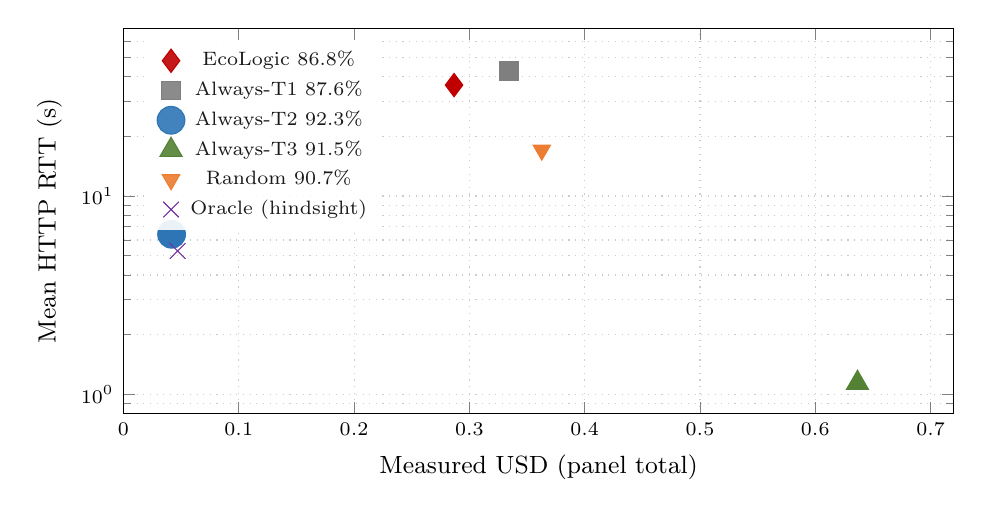
\begin{tikzpicture}
\begin{axis}[
  width=\columnwidth,
  height=2.55in,
  ymode=log,
  xmin=0, xmax=0.72,
  ymin=0.8, ymax=70,
  xlabel={Measured USD (panel total)},
  ylabel={Mean HTTP RTT (s)},
  grid=both,
  grid style={dotted,gray!40},
  legend style={font=\scriptsize, at={(0.03,0.97)}, anchor=north west, draw=none, fill=white, fill opacity=0.9},
  tick label style={font=\scriptsize},
  label style={font=\small},
  clip=false,
]
\addplot[only marks, mark=diamond*, mark size=4.2pt, color={rgb,255:red,192;green,0;blue,0}]
  coordinates {(0.28674677, 36.1967)};
\addlegendentry{EcoLogic 86.8\%}
\addplot[only marks, mark=square*, mark size=3.4pt, color={rgb,255:red,127;green,127;blue,127}]
  coordinates {(0.33422946, 42.4728)};
\addlegendentry{Always-T1 87.6\%}
\addplot[only marks, mark=*, mark size=5.0pt, color={rgb,255:red,46;green,117;blue,182}]
  coordinates {(0.0417509, 6.4132)};
\addlegendentry{Always-T2 92.3\%}
\addplot[only marks, mark=triangle*, mark size=4.6pt, color={rgb,255:red,84;green,130;blue,53}]
  coordinates {(0.636595, 1.1417)};
\addlegendentry{Always-T3 91.5\%}
\addplot[only marks, mark=triangle*, mark options={rotate=180}, mark size=3.6pt, color={rgb,255:red,237;green,125;blue,49}]
  coordinates {(0.36280891, 17.0225)};
\addlegendentry{Random 90.7\%}
\addplot[only marks, mark=x, mark size=4pt, color={rgb,255:red,112;green,48;blue,160}]
  coordinates {(0.04702266, 5.2842)};
\addlegendentry{Oracle (hindsight)}
\end{axis}
\end{tikzpicture}
\caption{Cost--latency scatter of policies. Marker size is qualitative with accuracy (Always-T2 largest among deployable points). Always-T2 and Always-T3 form the 2-D hull; EcoLogic is interior and 3-D-dominated by Always-T2.}
\label{fig:pareto}
\end{figure}

\subsection{Why the router loses on latency}
The keyword rule maps ``easy / general'' queries onto T1, intended as the cheap local default. In this substitute-model stack T1 is the \emph{slowest} service distribution, because Qwen3.5-9B writes long completions, not because it is a worse GPU. Over-predicting that a query should avoid the middle or frontier model is, operationally, a request to wait on T1's p90. A router cannot ``save latency'' by shifting mass onto a backend whose p90 is $16.7\times$ T2's p90 ($166.58/9.96$).

The oracle's mix ($343/364$ on T2) is independent confirmation that, under these prices and labels, the hindsight-correct cheap choice \emph{is} T2. Query-conditioned assignment had room only in the thin T1/T3 residual ($9+12$ items). The deployed heuristic used the opposite residual: it spent $274$ calls on T1.

\subsection{SLO attainment, not only means}
Interactive serving is an SLO problem. Table~\ref{tab:slo} reports the fraction of panel queries whose selected-tier HTTP RTT is $\le$ a deadline. Under a $10$\,s deadline, Always-T2 meets $90.1\%$ of queries and Always-T3 meets $100\%$; EcoLogic meets $44.5\%$. Under a $2$\,s interactive deadline, Always-T3 meets $87.1\%$ and EcoLogic meets $3.6\%$. Serial goodput (queries per hour if calls are issued one-at-a-time) is $99$ for EcoLogic, $561$ for Always-T2, and $3153$ for Always-T3. That quantity is not a multi-tenant throughput; it is the reciprocal of mean RTT, reported so that a $5.6\times$ mean-latency gap is not left as an abstract ratio.

A nonparametric paired sign test on per-query RTT versus Always-T2 rejects easily: EcoLogic is slower on $261/364$ queries, faster on $16$, and tied on $87$ (the $87$ are exactly the items already sent to T2). Two-sided $p=1.66\times 10^{-15}$. Ties are not evidence of routing skill; they are the T2 subset of the mix.

The slowest $10\%$ of EcoLogic queries ($37/364$) carry $54.4\%$ of selected-tier latency mass (Table~\ref{tab:tail}). Always-T2's corresponding tail is $41.5\%$ of a much smaller total; Always-T3's is $22.1\%$. A mean SLO that ignores that concentration will under-provision the replica that inherited T1.

Leave-one-benchmark-out (Table~\ref{tab:lob}) and a $21$-cell mix simplex on per-benchmark mean RTT: Always-T2 is faster and at least as accurate on all seven subsets and cheaper-in-time in $21/21$ mix cells. Item bootstrap ($10{,}000$ draws): Always-T2 dominates on accuracy and latency in $99.99\%$ of resamples. Service-time CVs are $1.34$ (T1), $2.06$ (T2; one $196$\,s HumanEval outlier), and $0.58$ (T3). A mean-based router SLO is therefore the wrong summary for T1, whose mean is already $2.36\times$ its median.

Percentile estimates are themselves noisy. A $5000$-resample bootstrap of p90 (seed $20260905$) gives EcoLogic $[70.39, 181.95]$\,s versus Always-T2 $[8.64, 11.26]$\,s. The intervals do not overlap. Always-T3's p90 interval is $[1.96, 2.28]$\,s.

\begin{table}[t]
\centering
\caption{Leave-one-benchmark-out and single-benchmark slices. Cost here is total selected-tier HTTP RTT (s). Always-T2 dominates EcoLogic on every subset; McNemar quality is HumanEval-driven.}
\label{tab:lob}
\setlength{\tabcolsep}{2.6pt}
\begin{tabular}{@{}lrrrrrr@{}}
\toprule
Subset & $n$ & Eco acc & T2 acc & Eco s & T2 s & McNemar \\
\midrule
all & 364 & 86.8\% & 92.3\% & 13176 & 2334 & $3.2\mathrm{e}{-4}$ \\
drop HumanEval & 200 & 88.0\% & 89.0\% & 6642 & 1023 & $0.73$ \\
only HumanEval & 164 & 85.4\% & 96.3\% & 6534 & 1312 & $1.2\mathrm{e}{-4}$ \\
only MMLU & 100 & 83\% & 84\% & 3493 & 397 & $1.0$ \\
only GSM8K & 100 & 93\% & 94\% & 3149 & 626 & $1.0$ \\
\bottomrule
\end{tabular}
\end{table}

\begin{table}[t]
\centering
\caption{Tail concentration: share of selected-tier latency mass in the slowest $10\%$ of queries ($k{=}37$).}
\label{tab:tail}
\setlength{\tabcolsep}{3.2pt}
\begin{tabular}{@{}lrrr@{}}
\toprule
Policy & mass in top $10\%$ & tail min s & tail mean s \\
\midrule
EcoLogic & 54.4\% & 108.58 & 193.8 \\
Always-T1 & 47.2\% & 166.58 & 197.2 \\
Always-T2 & 41.5\% & 9.96 & 26.2 \\
Always-T3 & 22.1\% & 2.12 & 2.49 \\
\bottomrule
\end{tabular}
\end{table}

\begin{table}[t]
\centering
\caption{SLO attainment: fraction of $n{=}364$ queries with selected-tier HTTP RTT $\le$ deadline. Serial q/h $=3600/$mean RTT (one-at-a-time; not multi-tenant). p90 bootstrap is a $95\%$ percentile interval, $5000$ resamples.}
\label{tab:slo}
\setlength{\tabcolsep}{2.8pt}
\begin{tabular}{@{}lrrrrrr@{}}
\toprule
Policy & $\le$2s & $\le$10s & $\le$30s & q/h & p90 [CI] \\
\midrule
EcoLogic & 3.6\% & 44.5\% & 72.3\% & 99 & 108.6 [70, 182] \\
Always-T1 & 0.0\% & 26.1\% & 64.0\% & 85 & 166.6 [76, 183] \\
Always-T2 & 13.7\% & 90.1\% & 98.4\% & 561 & 10.0 [8.6, 11.3] \\
Always-T3 & 87.1\% & 100\% & 100\% & 3153 & 2.1 [2.0, 2.3] \\
Random & 37.6\% & 73.1\% & 87.1\% & 211 & 43.3 [29, 61] \\
\bottomrule
\end{tabular}
\end{table}

\subsection{The loss is not one benchmark}
Policy mean RTT is high on every slice. EcoLogic: HumanEval $39.84$\,s (p90 $166.58$), MMLU $34.93$\,s (p90 $88.83$), GSM8K $31.49$\,s (p90 $75.07$). Always-T2 on the same slices: means $8.00$ / $3.97$ / $6.26$\,s (HumanEval p90 $11.03$). The router does not ``pay the T1 tail only on code.'' It pays it on multiple-choice and grade-school math as well, because the keyword default is T1.

Table~\ref{tab:slo_bench} splits SLO attainment the same way. Under a $10$\,s deadline EcoLogic is in on $47.6\%$ of HumanEval, $42\%$ of MMLU, and $42\%$ of GSM8K. Always-T2 is in on $86.6\%$ / $96\%$ / $90\%$. Always-T3 is in on $100\%$ of every slice at $10$\,s; the $2$\,s interactive bar is the one that separates T3 (HumanEval $96.3\%$, MMLU $97\%$, GSM8K $62\%$) from everyone else.

Completion length, not a slower decoder, is the demand. Mean seconds per output token are $11.94$\,ms (T1) and $12.74$\,ms (T2); Pearson $r$ of completion tokens versus \texttt{latency\_s} is $0.990$ / $0.998$ / $0.959$ on T1/T2/T3. Mean T1 completions are $3879$ / $3328$ / $3311$ tokens on HumanEval / MMLU / GSM8K; T2 is $668$ / $318$ / $495$. A router that classifies ``easy'' as ``send to the 9B reasoner'' is classifying into the longest decode on every benchmark (Fig.~\ref{fig:toklat}).

\begin{table}[t]
\centering
\caption{Per-benchmark SLO attainment (selected-tier HTTP RTT).}
\label{tab:slo_bench}
\setlength{\tabcolsep}{3.2pt}
\begin{tabular}{@{}llrrr@{}}
\toprule
Policy & Bench & $\le$2s & $\le$10s & $\le$30s \\
\midrule
EcoLogic & HumanEval & 1.8\% & 47.6\% & 66.5\% \\
         & MMLU & 7.0\% & 42\% & 72\% \\
         & GSM8K & 3.0\% & 42\% & 82\% \\
Always-T2 & HumanEval & 4.3\% & 86.6\% & 98.2\% \\
          & MMLU & 39\% & 96\% & 99\% \\
          & GSM8K & 4.0\% & 90\% & 98\% \\
Always-T3 & HumanEval & 96.3\% & 100\% & 100\% \\
          & MMLU & 97\% & 100\% & 100\% \\
          & GSM8K & 62\% & 100\% & 100\% \\
\bottomrule
\end{tabular}
\end{table}

\subsection{A labelled M/G/1 what-if}
\label{sec:mg1}
Table~\ref{tab:mg1} applies Pollaczek--Khinchine to the measured RTT distributions as if they were exclusive service times on a dedicated replica. This is \textbf{not} a fit to the HTTP trace: the stored $L$ already includes provider queueing, so adding an M/G/1 wait would double-count if treated as a forecast. It is a capacity statement about the \emph{mix}. EcoLogic's serial capacity is $99$\,q/h. At an offered $50$\,q/h the what-if sojourn is $99.6$\,s ($\rho{=}0.50$). Always-T2 at the same offered load is $8.06$\,s ($\rho{=}0.09$). At $90$\,q/h EcoLogic is near saturation ($\rho{=}0.90$, sojourn $633$\,s) while Always-T2 remains $9.62$\,s. At $200$\,q/h EcoLogic is unstable; Always-T2 is still stable ($\rho{=}0.36$, sojourn $15.7$\,s). Any offered load between $99$ and $561$\,q/h is infeasible for the deployed mix and feasible for Always-T2 even before a second replica is considered.

\begin{table}[t]
\centering
\caption{M/G/1 sojourn $E[T]{=}E[W]{+}E[S]$ if measured HTTP RTT were exclusive $S$ (Pollaczek--Khinchine, measured CV). \textbf{Hypothetical dedicated replica, not a prediction of the trace.} ``---'' means $\rho\ge 1$.}
\label{tab:mg1}
\setlength{\tabcolsep}{3.0pt}
\begin{tabular}{@{}lrrrr@{}}
\toprule
Policy & $10$\,q/h & $50$\,q/h & $90$\,q/h & $200$\,q/h \\
\midrule
EcoLogic & $43.2$\,s & $99.6$\,s & $633$\,s & --- \\
Always-T1 & $50.4$\,s & $128$\,s & --- & --- \\
Always-T2 & $6.72$\,s & $8.06$\,s & $9.62$\,s & $15.7$\,s \\
Always-T3 & $1.14$\,s & $1.15$\,s & $1.16$\,s & $1.19$\,s \\
\bottomrule
\end{tabular}
\end{table}

\begin{figure}[t]
\centering
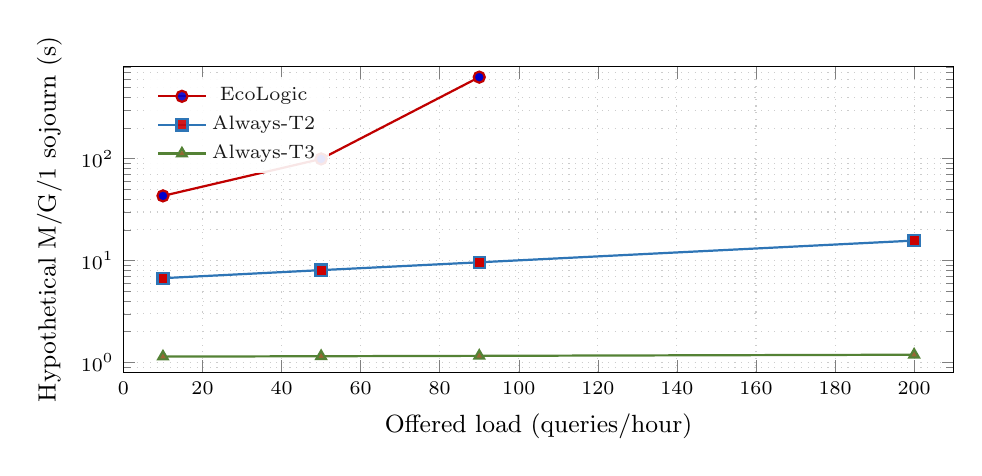
\begin{tikzpicture}
\begin{axis}[
  width=\columnwidth,
  height=2.15in,
  ymode=log,
  xmin=0, xmax=210,
  ymin=0.8, ymax=800,
  xlabel={Offered load (queries/hour)},
  ylabel={Hypothetical M/G/1 sojourn (s)},
  grid=both,
  grid style={dotted,gray!40},
  legend style={font=\scriptsize, at={(0.03,0.97)}, anchor=north west, draw=none, fill=white, fill opacity=0.9},
  tick label style={font=\scriptsize},
  label style={font=\small},
]
\addplot+[mark=*, thick, color={rgb,255:red,192;green,0;blue,0}]
  coordinates {(10,43.21) (50,99.64) (90,633.47)};
\addlegendentry{EcoLogic}
\addplot+[mark=square*, thick, color={rgb,255:red,46;green,117;blue,182}]
  coordinates {(10,6.72) (50,8.06) (90,9.62) (200,15.72)};
\addlegendentry{Always-T2}
\addplot+[mark=triangle*, thick, color={rgb,255:red,84;green,130;blue,53}]
  coordinates {(10,1.14) (50,1.15) (90,1.16) (200,1.19)};
\addlegendentry{Always-T3}
\end{axis}
\end{tikzpicture}
\caption{Labelled M/G/1 what-if sojourn versus offered load (log $y$). EcoLogic is omitted at $200$\,q/h ($\rho\ge 1$). Not a forecast of the HTTP trace: stored RTT is treated as exclusive $S$.}
\label{fig:mg1}
\end{figure}

\section{Answers to the research questions}

\textbf{RQ1.} No. Table~\ref{tab:tiers} and Fig.~\ref{fig:cdf} are three SLO classes, not three interchangeable backends. T3 is a $1$--$3$\,s interactive class. T2 is a $4$--$10$\,s class with a thin tail. T1 is a heavy-tailed minutes-scale class whose p90 is $16.7\times$ T2's. Seconds per output token do not explain the ranking; completion length does.

\textbf{RQ2.} No. The deployable 2-D hull under (USD, mean RTT) is \{Always-T2, Always-T3\}. EcoLogic is strictly interior, and Always-T2 additionally dominates it on accuracy. SLO attainment (Table~\ref{tab:slo}) and the labelled M/G/1 region (Fig.~\ref{fig:mg1}) agree: the router is not a latency tactic.

\textbf{RQ3.} No for latency and cost; partly for quality. Always-T2 is faster and cheaper on every leave-one-benchmark subset and in every mix-simplex cell. The paired accuracy rejection is HumanEval-driven (Table~\ref{tab:lob}). Dropping HumanEval does not save the router on seconds or dollars.

\begin{figure}[t]
\centering
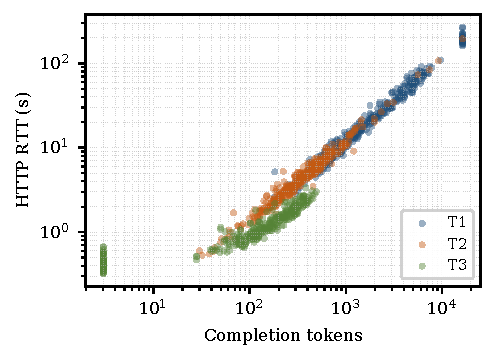
\includegraphics[width=\columnwidth]{artifacts/fig3_tokens_latency.pdf}
\caption{Completion tokens versus HTTP RTT (log--log). T1 and T2 lie on nearly the same seconds-per-token line; T1 is slow because it emits more tokens. T3 is short-decode and HTTP-overhead dominated.}
\label{fig:toklat}
\end{figure}

\section{Implications for LLMOps}

A serving organization that introduces a router has changed its workload mix. The performance question is not whether the classifier is clever; it is whether the induced mix improves the Pareto surface relative to static assignment.

\paragraph{Beat the empirically best static backend.}
On this price and latency vector, that backend is T2 for cost and T3 for latency. A router that does not appear on the hull has not earned its control loop. Cost-matched random mixtures and ``call-fraction matching'' are secondary; first, plot the static vertices.

\paragraph{Default-to-local is an SLO decision.}
If the default tier is a verbose open-weight model, most queries inherit that model's tail. Difficulty taxonomies that treat ``easy'' as ``send to the 9B'' can invert the latency ranking.

\paragraph{Percentiles before means.}
T1 mean $42$\,s vs.\ p50 $18$\,s is a reporting failure if an SLO is p90. Policy p90 (EcoLogic $109$\,s vs.\ Always-T2 $10$\,s) is the number an on-call engineer would page on.

\paragraph{Measure the classifier, but do not hide behind it.}
Our EcoLogic numbers \emph{omit} router-span time. The assignment mix alone is enough to lose. Adding a measured hop cannot reverse domination by Always-T2.

\paragraph{Token length is the hidden service demand.}
With $r\approx 0.99$ between completion tokens and RTT at T1/T2, admission control and routing that ignore expected decode length are incomplete.

\paragraph{Pick an SLO class, then pick a static vertex.}
Table~\ref{tab:slo} is the operational form of the Pareto plot. A $2$\,s interactive SLO has only Always-T3 as a feasible static policy on this panel. A $10$\,s SLO can use Always-T2 ($90.1\%$ in) and still beats the router ($44.5\%$ in). A router that is interior on USD$\times$mean RTT is usually interior on SLO attainment too; checking one table is cheaper than shipping the classifier.

\paragraph{HTTP RTT is still a serving metric.}
TTFT, GPU occupancy, and isolated decode time were not recorded. Full-request RTT is nonetheless what a synchronous API client waits for, and it is what the stored \texttt{latency\_s} field is. For SLO design of non-streaming Q\&A---EcoLogic's actual product shape---RTT is the right first measurement. Streaming products need TTFT as a second axis; that is future work, not a reason to ignore a $10\times$ p90 gap.

\paragraph{Tail at scale is a mix problem.}
The slowest $10\%$ of EcoLogic queries are $54\%$ of its latency mass. Dean and Barroso's warning about rare delays becoming typical under fan-out~\cite{dean2013tail} applies here without fan-out: a classifier that over-uses a heavy-tailed backend \emph{creates} the tail the rest of the stack will see.

\paragraph{Capacity follows the mix.}
Serial goodput is $99$\,q/h for EcoLogic versus $561$\,q/h for Always-T2. The labelled M/G/1 what-if (Table~\ref{tab:mg1}) turns that ratio into a stability region: loads that are trivial for Always-T2 saturate the deployed mix. We do not simulate a multi-tenant queue (Section~\ref{sec:threats}); the inequality already follows from the measured means and CVs.

\paragraph{Do not shop prompt surfaces.}
A wrapped-instruction variant of the same keyword rule exists in the artifact (mix $137/53/174$, mean RTT $18.52$\,s, p90 $34.98$\,s, \$0.440, accuracy $89.6\%$). It is faster than production raw routing because it escalates HumanEval to T3, and it is still strictly slower and more expensive than Always-T2. We do not promote it. Surface choice is a researcher degree of freedom that moves mean RTT by $2\times$; locking the production surface before seeing latency is part of a competent evaluation.

\paragraph{A minimum latency report for a $k$-backend router.}
(1)~Per-backend RTT distribution with p50/p90/p99, and a sentence stating TTFT vs.\ full RTT.
(2)~Policy latency as the empirical mix of \emph{selected} calls, not mix$\times$mean of backend averages.
(3)~SLO attainment at the product deadline, plus serial goodput $3600/\mathrm{mean}$.
(4)~The $k$ static backends on the same plot; domination is with respect to those vertices.
(5)~Classifier-span time, or an explicit $n_{\mathrm{measured}}=0$ if it was not recorded.
(6)~Tail mass (share of seconds in the slowest $10\%$) and, if a queueing formula is shown, an explicit label that stored RTT is not exclusive service time.

\section{Threats to Validity}
\label{sec:threats}

\paragraph{HTTP RTT $\neq$ TTFT $\neq$ GPU time.}
Interactive products care about TTFT and token streaming. We did not record them. Rankings could change if T1 streams useful tokens early while T2 does not---untested.

\paragraph{No concurrent load.}
Calls are offline, not a multi-tenant trace. Queueing at a shared replica is inside provider RTT but we do not control offered load, batch size, or prefix-cache hit rate. p99 under deadlock-level concurrency is unmeasured.

\paragraph{In-sample keyword routing.}
The heuristic is scored on the same $n{=}364$ used to inspect it. Always-T2 is an in-sample static vertex (unconditional means on the eval set). Both facts bias \emph{toward} finding some routing win; we still find a loss.

\paragraph{Substitute models.}
Original Together slugs were retired. Qwen3.5-9B's long completions may not match the intended T1. The measurement is of the stack that was actually called.

\paragraph{Unmeasured router overhead.}
$364/364$ classifier spans missing. Production EcoLogic latency is a lower bound on a deployed router.

\paragraph{No cloud deployment.}
\texttt{deployment\_real\_v2} in the repository is a local stub dry-run, not Cloud Run or Lambda. We do not claim a paid serverless experiment.

\paragraph{What would reverse the result.}
Four changes could put EcoLogic on the hull. (1)~A T1 that emits T2-like completions: mean T1 length is $6.8\times$ T2, and $r{=}0.99$ with RTT, so a non-reasoning 9B could collapse T1 into T2's SLO class. The retired production slug may have been that model; this panel is not. (2)~A classifier whose mix matches the oracle ($9/343/12$) rather than $274/87/3$. Headroom exists ($96.4\%$ oracle accuracy, mean $5.28$\,s) but the deployed rule uses the opposite residual. (3)~A TTFT ranking that inverts T1 versus T2 while full RTT does not---unmeasured. (4)~A production mix with almost no HumanEval-like items does \emph{not} reverse latency or USD domination (Table~\ref{tab:lob}); it only removes the McNemar rejection. Concurrent load that saturates T2 while leaving T1 idle is theoretically possible and untested; it would have to overcome a $5.6\times$ mean-RTT gap.

\paragraph{Simulated serverless DES and M/G/1 (not used as measurement).}
A discrete-event path replays stored HTTP RTTs as exclusive service times and then adds queue wait. Because those RTTs already include provider queueing, the simulation double-counts delay. Idle timeout and cold-start extra are config knobs, not platform observations. We omit those sojourn times from headline tables. The Pollaczek--Khinchine numbers in Table~\ref{tab:mg1} are the same object stated as a formula, and are labelled hypothetical.

\paragraph{Oracle is hindsight.}
Using labels to pick the cheapest correct tier is an upper bound, not a policy.

\paragraph{Accuracy metric.}
Objective graders (code execution, exact match). Chat quality and judge-LM scores~\cite{stoica2024lmsys} are out of scope.

\section{Conclusion}

Query-conditioned LLM assignment is a scheduler. On a frozen 364-item, three-backend panel, a deployed keyword router does not improve the cost--latency--accuracy Pareto set. It over-assigns the slow, long-tailed backend (T1 mean $42.47$\,s, p90 $166.58$\,s), producing policy p90 $108.58$\,s at \$0.2867 and $86.8\%$ accuracy. Always-T2 is cheaper, faster at every reported percentile except that T2 still has a rare $196$\,s outlier, and more accurate. Always-T3 occupies the low-latency vertex. The hull is those two static policies.

The LLMOps baseline is therefore simple: measure per-backend latency \emph{distributions}, assign everything to the vertex that matches the SLO, and require any router to move the empirical mix onto the hull---not into T1's tail. Routing is not free, even when the classifier clock is not running.

\section*{Data availability}
All digits reconstruct from committed \texttt{raw\_results/graded.jsonl} and \texttt{routing.json} via \texttt{papers/aiperf/analysis.py}. Wall-clock cross-checks match \texttt{woais\_experiments/results/latency/stage12\_wallclock.json} and \texttt{frontier\_per\_query.csv}. No new API calls.

\bibliographystyle{IEEEtran}
\bibliography{refs}

\end{document}
